%!TEX root = main.tex

\subsection{Proof of Lemma~\ref{lemma_actives_sets}}

Since the objective function $\Psi_{\kappa}$ is convex with respect to $(u,v)$, the set of optima of problem~\eqref{screen-sinkhorn} is non empty.
Introducing two dual variables $\lambda \in \R^n_{+}$ and $\beta \in \R^m_{+}$ for each constraint, the Lagrangian of problem~\eqref{screen-sinkhorn} reads as 
\begin{equation*}
  \mathscr{L}(u,v, \lambda, \beta) = \frac \varepsilon\kappa\inr{\lambda, \mathbf{1}_n} + \varepsilon\kappa\inr{\beta, \mathbf{1}_m} + \mathbf{1}_n^\top B(u,v) \mathbf{1}_m - \inr{\kappa u, \mu} - \inr{\frac v\kappa, \nu} -\inr{\lambda,e^{u}} - \inr{\beta,e^{v}}
\end{equation*}
First order conditions then yield that the Lagrangian multiplicators solutions $\lambda^{*}$ and $\beta^{*}$ satisfy 
\begin{align*}
  &\nabla_u\mathscr{L}(u^{*},v^{*}, \lambda^{*}, \beta^{*})=  e^{u^{*}} \odot(Ke^{v^{*}} - \lambda^{*}) - \kappa\mu = \mathbf 0_n,\\
  & \text{ and } \nabla_v\mathscr{L}(u^{*},v^{*}, \lambda^{*}, \beta^{*})=  e^{v^{*}} \odot(K^\top e^{u^{*}} - \beta) - \frac \nu\kappa = \mathbf 0_m
\end{align*}
which leads to 
\begin{align*}
  &\lambda^{*} = K e^{v^{*}} - \kappa\mu \oslash e^{u^{*}} \text{ and }
  \beta^{*} = K^\top e^{u^{*}} - \nu \oslash \kappa e^{v^{*}}
\end{align*}

For all $i=1, \ldots, n$ we have that $e^{u^{*}_i} \geq \varepsilon\kappa^{-1}$. Further, the condition on the dual variable $\lambda^{*}_i > 0$  ensures that $e^{u^{*}_i} = \varepsilon\kappa^{-1}$ and hence $i \in I^\complement_{\varepsilon,\kappa}$. We have that $\lambda^{*}_i > 0$ is equivalent to $e^{u^{*}_i}r_i(K) e^{v^{*}_j} >  \kappa{\mu_i}$ which  is satisfied when $\varepsilon^2r_i(K) >  \kappa{\mu_i}.$  
In a symmetric way we can prove the same statement for $e^{v^{*}_j}$.

\subsection{Proof of Proposition~\ref{prop:bounds_of_usc_and_vsc}}

We prove only the first statement~\eqref{bound_on_u} and similarly we can prove the second one~\eqref{bound_on_v}.
For all $i\in I_{\varepsilon,\kappa}$, we have $e^{u^{\text{sc}}_i} > \frac \varepsilon\kappa$ or $e^{u^{\text{sc}}_i} = \frac \varepsilon\kappa$. In one hand, if $e^{u^{\text{sc}}_i} > \frac \varepsilon\kappa$ then according to the optimality conditions $\lambda^{\text{sc}}_i = 0,$ which implies $e^{u^{\text{sc}}_i} \sum_{j=1}^m K_{ij} e^{v^{\text{sc}}_j} = \kappa\mu_i$.
In another hand, we have 
\begin{align*}
e^{u^{\text{sc}}_i} \min_{i,j}K_{ij} \sum_{j=1}^m e^{v^{\text{sc}}_j} \leq e^{u^{\text{sc}}_i} \sum_{j=1}^m K_{ij} e^{v^{\text{sc}}_j} = \kappa\mu_i.
\end{align*}
We further observe that $\sum_{j=1}^m e^{v^{\text{sc}}_j} = \sum_{j \in J_{\varepsilon,\kappa}} e^{v^{\text{sc}}_j} + \sum_{j \in J^\complement_{\varepsilon,\kappa}} e^{v^{\text{sc}}_j} \geq \varepsilon\kappa |J_{\varepsilon,\kappa}| + \varepsilon\kappa |J^\complement_{\varepsilon,\kappa}|=\varepsilon\kappa m.$ Then
\begin{equation*}
\max_{i\in I_{\varepsilon,\kappa}} e^{u^{\text{sc}}_i} \leq \frac \varepsilon\kappa \vee \frac{\max_{i\in I_{\varepsilon,\kappa}}\mu_i}{m\varepsilon K_{\min}} \leq \frac \varepsilon\kappa \vee \frac{\max_{i\in I_{\varepsilon,\kappa}}\mu_i}{m\varepsilon K_{\min}}.
\end{equation*}
Analogously, one can obtain for all $j\in J_{\varepsilon,\kappa}$
\begin{equation}
\label{upper_bound_v_potential}
\max_{j\in J_{\varepsilon,\kappa}}e^{v^{\text{sc}}_j} \leq \varepsilon\kappa \vee \frac{\max_{j \in J_{\varepsilon,\kappa}} \nu_j}{n\varepsilon K_{\min}} \leq \varepsilon\kappa \vee \frac{\max_{j \in J_{\varepsilon,\kappa}} \nu_j}{n\varepsilon K_{\min}} .
\end{equation}

Now, since $K_{ij} \leq 1$, we have 
\begin{align*}
e^{u^{\text{sc}}_i} \sum_{j=1}^m e^{v^{\text{sc}}_j} \geq e^{u^{\text{sc}}_i} \sum_{j=1}^m K_{ij}e^{v^{\text{sc}}_j} = \kappa\mu_i.
\end{align*}
Using~\eqref{upper_bound_v_potential}, we get 
\begin{align*}
\sum_{j=1}^m e^{v^{\text{sc}}_j} &= \sum_{j \in J_{\varepsilon,\kappa}} e^{v^{\text{sc}}_j} + \sum_{j \in J^\complement_{\varepsilon,\kappa}} e^{v^{\text{sc}}_j}
\leq \varepsilon\kappa |J^\complement_{\varepsilon,\kappa}| + \varepsilon\kappa \vee \frac{\max_{j\in J_{\varepsilon,\kappa}} \nu_j}{n\varepsilon K_{\min}} |J_{\varepsilon,\kappa}|.
\end{align*}
Therefore,
\begin{align*}
\min_{i \in I_{\varepsilon,\kappa}} e^{u^{\text{sc}}_i}  \geq \frac \varepsilon\kappa \vee \frac{\kappa\min_{I_{\varepsilon,\kappa}}\mu_i}{\varepsilon\kappa (m-m_b) + \varepsilon\kappa \vee \frac{\max_{j\in J_{\varepsilon,\kappa}} \nu_j}{n\varepsilon K_{\min}} m_b}.
\end{align*}

\subsection{Proof of Proposition~\ref{proposition_error_in_marginals}}

We define the distance function $\varrho: \R_+ \times \R_+ \mapsto [0, \infty]$ by $\varrho(a,b) = b - a + a \log(\frac ab).$
While $\varrho$ is not a metric, it is easy to see that $\varrho$ is not nonnegative and satisfies $\varrho(a,b) =0$ iff $a=b$.
The violations are computed through the following function: 
\begin{equation*}
	d_{\varrho}(\gamma,\beta) = \sum_{i=1}^n \varrho(\gamma_i,\beta_i), \text{ for } \gamma, \beta \in \R^n_+.
\end{equation*}
Note that if $\gamma,\beta$ are two vectors of positive entries, $d_{\varrho}(\gamma,\beta)$ will return some measurement on how far they are from each other. The next Lemma is from~\cite{khalilabid2018} (see Lemma 7 herein).
\begin{lemma}
\label{lem:pinsker}
For any $\gamma, \beta \in \R^n_+$, the following generalized Pinsker inequality holds 
\begin{align*}
\norm{\gamma - \beta}_1 \leq \sqrt{7 (\norm{\gamma}_1\wedge \norm{\beta}_1)d_{\varrho}(\gamma,\beta)}.
\end{align*}
\end{lemma}

The optimality conditions for $({u}^{\text{sc}}, {v}^{\text{sc}})$ entails 
\begin{align}
\label{i-th-marginal-mu} 
{\mu}^{\text{sc}}_i  &= 
\begin{cases}
e^{u^{\text{sc}}_i} \sum_{j=1}^m K_{ij} e^{v^{\text{sc}}_j}, \text{ if  }i \in I_{\varepsilon,\kappa},\\
\frac \varepsilon\kappa\sum_{j=1}^m K_{ij} e^{v^{\text{sc}}_j}, \text{ if  }i \in I^\complement_{\varepsilon,\kappa}
\end{cases}
=\begin{cases}
\kappa \mu_i, \text{ if  }i \in I_{\varepsilon,\kappa},\\
\frac \varepsilon\kappa\sum_{j=1}^m K_{ij} e^{v^{\text{sc}}_j}, \text{ if  }i \in I^\complement_{\varepsilon,\kappa},
\end{cases}
\end{align}
and 
\begin{align}
\label{i-th-marginal-nu} 
{\nu}^{\text{sc}}_j  &= 
\begin{cases}
e^{v^{\text{sc}}_j} \sum_{i=1}^n K_{ij} e^{u^{\text{sc}}_i}, \text{ if  }j \in J_{\varepsilon,\kappa},\\
\varepsilon\kappa\sum_{i=1}^n K_{ij} e^{u^{\text{sc}}_i}, \text{ if  }j \in J^\complement_{\varepsilon,\kappa}
\end{cases}
=\begin{cases}
\frac{\nu_j}{\kappa}, \text{ if  }j \in J_{\varepsilon,\kappa},\\
\varepsilon\kappa\sum_{i=1}^n K_{ij} e^{u^{\text{sc}}_i}, \text{ if  }j \in J^\complement_{\varepsilon,\kappa}.
\end{cases}
\end{align}

By~\eqref{i-th-marginal-mu}, we have
\begin{align*}
d_\varrho({\mu} ,{\mu}^{\text{sc}}) &= \sum_{i=1}^n  {\mu}^{\text{sc}}_i - {\mu}_i + {\mu}_i  \log\Big(\frac{{\mu}_i}{{\mu}^{\text{sc}}_i }\Big)\\
&= \sum_{i\in I_{\varepsilon,\kappa}} (\kappa-1)\mu_i - \mu_i\log(\kappa) + \sum_{i\in I^\complement_{\varepsilon,\kappa}}\frac \varepsilon\kappa\sum_{j=1}^m K_{ij} e^{v^{\text{sc}}_j} - \mu_i + \mu_i \log\Big(\frac{\mu_i}{\frac \varepsilon\kappa\sum_{j=1}^m K_{ij} e^{v^{\text{sc}}_j}}\Big)\\
&= \sum_{i\in I_{\varepsilon,\kappa}} (\kappa-\log(\kappa)-1)\mu_i  + \sum_{i\in I^\complement_{\varepsilon,\kappa}}\frac \varepsilon\kappa\sum_{j=1}^m K_{ij} e^{v^{\text{sc}}_j} - \mu_i + \mu_i \log\Big(\frac{\mu_i}{\frac \varepsilon\kappa\sum_{j=1}^m K_{ij} e^{v^{\text{sc}}_j}}\Big).
\end{align*}
Now by~\eqref{bound_on_v}, we have in one hand 
\begin{align*}
\sum_{i\in I^\complement_{\varepsilon,\kappa}}\frac \varepsilon\kappa\sum_{j=1}^m K_{ij} e^{v^{\text{sc}}_j}&= \sum_{i\in I^\complement_{\varepsilon,\kappa}}\frac \varepsilon\kappa \Big(\sum_{j\in J_{\varepsilon,\kappa}}K_{ij} e^{v^{\text{sc}}_j} + \varepsilon \kappa\sum_{j\in J^\complement_{\varepsilon,\kappa}}K_{ij}\Big)\\
&\leq \sum_{i\in I^\complement_{\varepsilon,\kappa}}\frac \varepsilon\kappa \Big(m_b \max_{i,j}K_{ij}\frac{\max_{j \in J_{\varepsilon,\kappa}} \nu_j}{n\varepsilon K_{\min}} + (m - m_b)\varepsilon\kappa\max_{i,j}K_{ij}\Big) \\
&\leq (n-n_b)\Big(\frac{m_b\max_{j} \nu_j}{n\kappa K_{\min}} + (m- m_b) \varepsilon^2\Big).
\end{align*}
On the other hand, we get
\begin{align*}
\frac \varepsilon\kappa\sum_{j=1}^m K_{ij} e^{v^{\text{sc}}_j}&=\frac \varepsilon\kappa \Big(\sum_{j\in J_{\varepsilon,\kappa}}K_{ij} e^{v^{\text{sc}}_j} + \varepsilon \kappa\sum_{j\in J^\complement_{\varepsilon,\kappa}}K_{ij}\Big)\\
&\geq m_bK_{\min} \frac{m\varepsilon^2K_{\min}\min_{j \in J_{\varepsilon,\kappa}}\nu_j}{\kappa((n-n_b)m\varepsilon^2K_{\min} + m\varepsilon^2K_{\min} + n_b\kappa\max_{i\in I_{\varepsilon,\kappa}}\mu_i)}\\
&\qquad +\varepsilon^2 (m- m_b) K_{\min}\\
&\geq \frac{mm_b\varepsilon^2(K_{\min})^2\min_{j \in J_{\varepsilon,\kappa}}\nu_j}{\kappa((n-n_b)m\varepsilon^2K_{\min}+ m\varepsilon^2K_{\min} + n_b\kappa\max_{i\in I_{\varepsilon,\kappa}}\mu_i)}\\
&\qquad +\varepsilon^2 (m- m_b) K_{\min}\\
&\geq \frac{mm_b\varepsilon^2K_{\min}^2\min_{j \in J_{\varepsilon,\kappa}}\nu_j}{\kappa((n-n_b)m\varepsilon^2K_{\min}+ m\varepsilon^2K_{\min} + n_b\kappa\max_{i\in I_{\varepsilon,\kappa}}\mu_i)}.
\end{align*}
Then 
\begin{align*}
\frac{1}{\frac \varepsilon\kappa\sum_{j=1}^m K_{ij} e^{v^{\text{sc}}_j}} &\leq \frac{\kappa((n-n_b)m\varepsilon^2K_{\min}+ m\varepsilon^2K_{\min} + n_b\kappa\max_{i\in I_{\varepsilon,\kappa}}\mu_i)}{mm_b\varepsilon^2 K_{\min}^2\min_{j \in J_{\varepsilon,\kappa}}\nu_j}\\
&\leq \frac{\kappa(n-n_b+ 1)}{m_bK_{\min}\min_{j \in J_{\varepsilon,\kappa}}\nu_j} + \frac{n_b\kappa^2\max_{i\in I_{\varepsilon,\kappa}}\mu_i}{mm_b\varepsilon^2K_{\min}^2\min_{j \in J_{\varepsilon,\kappa}}\nu_j}.
\end{align*}
It entails 
\begin{align*}
&\sum_{i\in I^\complement_{\varepsilon,\kappa}}\frac \varepsilon\kappa\sum_{j=1}^m K_{ij} e^{v^{\text{sc}}_j} - \mu_i + \mu_i \log\Big(\frac{\mu_i}{\frac \varepsilon\kappa\sum_{j=1}^m K_{ij} e^{v^{\text{sc}}_j}}\Big)\\
&\qquad \leq (n-n_b)\bigg(\frac{m_b}{n\kappa K_{\min}} + (m- m_b) \varepsilon^2 - \min_{i}\mu_i\\
&\qquad \qquad + \max_{i}\mu_i\log\Big(\frac{\kappa(n-n_b+ 1)\max_{i}\mu_i}{m_bK_{\min}\min_{j \in J_{\varepsilon,\kappa}}\nu_j} + \frac{n_b\kappa^2(\max_{i}\mu_i)^2}{mm_b\varepsilon^2 K_{\min}^2\min_{j \in J_{\varepsilon,\kappa}}\nu_j}\Big)
\bigg).
\end{align*}
Therefore
\begin{align*}
d_\varrho({\mu},{\mu}^{\text{sc}}) &\leq n_b c_{\kappa}\max_{i} \mu_i + (n-n_b)\bigg(\frac{m_b\max_{j}\nu_j}{n\kappa K_{\min}} + (m- m_b) \varepsilon^2 - \min_{i}\mu_i\\
&\qquad + \max_{i} \mu_i\log\Big(\frac{\kappa(n-n_b+ 1)\max_{i} \mu_i}{m_bK_{\min}\min_{j \in J_{\varepsilon,\kappa}}\nu_j} + \frac{n_b\kappa^2(\max_{i} \mu_i)^2}{mm_b\varepsilon^2 K_{\min}^2\min_{j \in J_{\varepsilon,\kappa}}\nu_j}\Big).
\end{align*}
Finally, by Lemma~\ref{lem:pinsker} we obtain
\begin{align*}
\norm{{\mu} -{\mu}^{\text{sc}}}^2_1 \leq & n_bc_{\kappa}\max_{i} \mu_i + 7(n-n_b)\bigg(\frac{m_b\max_{j}\nu_j}{n\kappa K_{\min}} + (m- m_b) \varepsilon^2 - \min_{i}\mu_i\\
&+ \max_{i} \mu_i\log\Big(\frac{\kappa(n-n_b+ 1)\max_{i} \mu_i}{m_bK_{\min}\min_{j \in J_{\varepsilon,\kappa}}\nu_j} + \frac{n_b\kappa^2(\max_{i} \mu_i)^2}{mm_b\varepsilon^2K_{\min}^2\min_{j \in J_{\varepsilon,\kappa}}\nu_j}\Big).
\end{align*}
Following the same lines as above, we also have
\begin{align*}
\norm{{\nu} -{\nu}^{\text{sc}}}^2_1 \leq & m_bc_{\frac 1\kappa}\max_{i} \mu_i + 7(m-m_b)\bigg(\frac{n_b\kappa\max_{i}\mu_i}{mK_{\min}} + (n- n_b) \varepsilon^2 - \min_{j}\nu_j\\
&+ \max_{j} \nu_j\log\Big(\frac{(m-m_b+ 1)\max_{j} \nu_j}{n_b\kappa K_{\min}\min_{i \in I_{\varepsilon,\kappa}}\mu_i} + \frac{m_b(\max_{j} \nu_j)^2}{nn_b\varepsilon^2\kappa^2K_{\min}^2\min_{i \in I_{\varepsilon,\kappa}}\mu_i}\Big).%\bigg\}^{1/2}
\end{align*}
To get the closed forms~\eqref{marginal-error-mu} and~\eqref{marginal-error-nu}, we used the follwoing facts:
\begin{remark}
\label{rem:orders_of_epsilonappa}
 We have 
$\varepsilon = \bigO((mnK_{\min}^2)^{-1/4})$, $\kappa= \bigO(\sqrt{m/(nc_{\mu\nu}K_{\min})}),$ $\kappa^{-1} = \bigO(\sqrt{n/(mK_{\min}c_{\mu\nu}})$, $(\kappa/\varepsilon)^2 = \bigO( m^{3/2} / \sqrt{nK_{\min}}(c_{\mu\nu})^{3/2})$, and $(\varepsilon\kappa)^{-2} = \bigO(n^{3/2}/\sqrt{mK_{\min}}c^{3/2}_{\mu\nu}).$
\end{remark}

\subsection{Proof of Proposition~\ref{prop:objective-error}}

We first define $\widetilde{K}$ a rearrgement of $K$ with respect to the active sets $I_{\varepsilon,\kappa}$ and $J_{\varepsilon,\kappa}$as follows:
\begin{equation*}
\widetilde{K} = 
\begin{bmatrix}
K_{(I_{\varepsilon,\kappa}, J_{\varepsilon,\kappa})} & K_{(I_{\varepsilon,\kappa}, J^\complement_{\varepsilon,\kappa})}\\
K_{(I^\complement_{\varepsilon,\kappa}, J_{\varepsilon,\kappa})} &K_{(I^\complement_{\varepsilon,\kappa}, J^\complement_{\varepsilon,\kappa})}
\end{bmatrix}.
\end{equation*}
Setting $\dt{\mu} = (\mu_{I_{\varepsilon,\kappa}}^\top, \mu_{I^\complement_{\varepsilon,\kappa}}^\top)^\top$, $\dt{\nu} = (\nu_{J_{\varepsilon,\kappa}}^\top, \nu_{J^\complement_{\varepsilon,\kappa}}^\top)^\top$ and for each vectors $u \in \R^n$ and $v\in \R^m$ we set $\dt{u} =(u_{I_{\varepsilon,\kappa}}^\top, u_{I^\complement_{\varepsilon,\kappa}}^\top)^\top  \text{ and } \dt{v} =(v_{J_{\varepsilon,\kappa}}^\top, v_{J^\complement_{\varepsilon,\kappa}}^\top)^\top.$
We then have 
\begin{equation*}
\Psi_{\varepsilon, \kappa} (u,v) = \mathbf 1_n^\top \widetilde{K}(\dt{u}, \dt{v}) \mathbf 1_m - \kappa \dt{\mu}^\top \dt{u} - \kappa^{-1} \dt{\nu}^\top \dt{v},
\end{equation*}
and 
\begin{equation*}
\Psi_{} (u,v) = \mathbf 1_n^\top \widetilde{K}(\dt{u}, \dt{v}) \mathbf 1_m - \dt{\mu}^\top \dt{u} - \dt{\nu}^\top \dt{v},
\end{equation*}
where
\begin{equation*}
  \widetilde{B}(\dt{u}, \dt{v}) = \Delta(e^{\dt{u}})\widetilde{K} \Delta(e^{\dt{v}}).
\end{equation*}
Let us consider the convex function
\begin{equation*}
	(\hat u, \hat v) \mapsto \inr{\mathbf 1_n, \widetilde{B}(\dt{\hat u}^{\text{}} ,\dt{\hat v}^{\text{}})\mathbf 1_m} - \inr{\kappa\dt{\hat u}, \widetilde{B}(\dt{u}^{\text{sc}} ,\dt{v}^{\text{sc}})\mathbf 1_m} - \inr{\kappa^{-1}\dt{\hat v}, \widetilde{B}(\dt{u}^{\text{sc}} ,\dt{v}^{\text{sc}})^\top\mathbf 1_n}.
\end{equation*}
Gradient inequality of any convex function g at point $x_o$ reads as $g(x_o) \geq g(x) + \inr{\nabla g(x), x_o - x}, \text{ for all } x \in \textbf{dom}(g).$
Applying the latter fact to the above function at point ($u^{\star}, v^{\star})$ we obtain
\begin{align*}
\inr{\mathbf 1_n, \widetilde{B}(\dt{u}^{\text{sc}} ,\dt{v}^{\text{sc}})\mathbf 1_m} &- \inr{\kappa\dt{u}^{\text{sc}}, \widetilde{B}(\dt{u}^{\text{sc}} ,\dt{v}^{\text{sc}})\mathbf 1_m} - \inr{\kappa^{-1}\dt{v}^{\text{sc}}, \widetilde{B}(\dt{u}^{\text{sc}} ,\dt{v}^{\text{sc}})^\top\mathbf 1_n}\\
& - \big(\inr{\mathbf 1_n, \widetilde{B}(\dt{u}^{\star} ,\dt{v}^{\star})\mathbf 1_m}  
- \inr{\kappa\dt{u}^{\star{}}, \widetilde{B}(\dt{u}^{\text{sc}} ,\dt{v}^{\text{sc}})\mathbf 1_m} 
- \inr{\kappa^{-1}\dt{v}^\star, \widetilde{B}(\dt{u}^{\text{sc}} ,\dt{v}^{\text{sc}})^\top\mathbf 1_n} \big)\\
&\qquad \qquad  \leq \inr{\dt{u}^{\text{sc}} - \dt{u}^\star, (1-\kappa) \widetilde{B}(\dt{u}^{\text{sc}} ,\dt{v}^{\text{sc}})\mathbf 1_m} 
+ \inr{\dt{v}^{\text{sc}} - \dt{v}^\star, (1-\kappa^{-1}) \widetilde{B}(\dt{u}^{\text{sc}} ,\dt{v}^{\text{sc}})^\top\mathbf 1_n}.
\end{align*}
Moreover,
\begin{align*}
\Psi_{\varepsilon, \kappa} (u^{\text{sc}} ,v^{\text{sc}}) -\Psi(u^\star, v^\star)
&= \inr{\mathbf 1_n, \widetilde{B}(\dt{u}^{\text{sc}} ,\dt{v}^{\text{sc}})\mathbf 1_m} - \inr{\kappa\dt{u}^{\text{sc}}, \widetilde{B}(\dt{u}^{\text{sc}} ,\dt{v}^{\text{sc}})\mathbf 1_m} - \inr{\kappa^{-1}\dt{v}^{\text{sc}}, \widetilde{B}(\dt{u}^{\text{sc}}, \dt{v}^{\text{sc}})\mathbf 1_n^\top}\\
&\qquad - \big( 
\inr{\mathbf 1_n, \widetilde{B}(\dt{u}^{\star} ,\dt{v}^{\star})\mathbf 1_m}  
- \inr{\dt{u}^{\star{}}, \widetilde{B}(\dt{u}^{\text{sc}} ,\dt{v}^{\text{sc}})\mathbf 1_m} 
- \inr{\dt{v}^\star, \widetilde{B}(\dt{u}^{\text{sc}} ,\dt{v}^{\text{sc}})^\top\mathbf 1_n} \big)\\
&\qquad + \inr{\kappa \dt{u}^{\text{sc}} - \dt{u}^{\star}, \widetilde{B}(\dt{u}^{\text{sc}} ,\dt{v}^{\text{sc}})\mathbf 1_m - \dt{\mu}} + \inr{\kappa^{-1}\dt{v}^{\text{sc}} - \dt{v}^{\star}, \widetilde{B}(\dt{u}^{\text{sc}} ,\dt{v}^{\text{sc}})^\top\mathbf 1_n - \dt{\nu}}.
\end{align*}
Hence,
\begin{align*}
\Psi_{\varepsilon, \kappa} (u^{\text{sc}} ,v^{\text{sc}}) -\Psi(u^\star, v^\star)
+& \big( \inr{\mathbf 1_n, \widetilde{B}(\dt{u}^{\star} ,\dt{v}^{\star})\mathbf 1_m} \\
&- \inr{\dt{u}^{\star{}}, \widetilde{B}(\dt{u}^{\text{sc}} ,\dt{v}^{\text{sc}})\mathbf 1_m} 
- \inr{\dt{v}^\star, \widetilde{B}(\dt{u}^{\text{sc}} ,\dt{v}^{\text{sc}})^\top\mathbf 1_n} \big)\\
& \qquad -\inr{\kappa \dt{u}^{\text{sc}} - \dt{u}^{\star}, \widetilde{B}(\dt{u}^{\text{sc}} ,\dt{v}^{\text{sc}})\mathbf 1_m - \dt{\mu}} -\inr{\kappa^{-1}\dt{v}^{\text{sc}} - \dt{v}^{\star}, \widetilde{B}(\dt{u}^{\text{sc}} ,\dt{v}^{\text{sc}})^\top\mathbf 1_n - \dt{\nu}}\\
& \leq \inr{\dt{u}^{\text{sc}} - \dt{u}^\star, (1-\kappa) \widetilde{B}(\dt{u}^{\text{sc}} ,\dt{v}^{\text{sc}})\mathbf 1_m} 
+ \inr{\dt{v}^{\text{sc}} - \dt{v}^\star, (1-\kappa^{-1}) \widetilde{B}(\dt{u}^{\text{sc}} ,\dt{v}^{\text{sc}})^\top\mathbf 1_n}\\
&\qquad + \big(\inr{\mathbf 1_n, \widetilde{B}(\dt{u}^{\star} ,\dt{v}^{\star})\mathbf 1_m}  
- \inr{\kappa\dt{u}^{\star{}}, \widetilde{B}(\dt{u}^{\text{sc}} ,\dt{v}^{\text{sc}})\mathbf 1_m} 
- \inr{\kappa^{-1}\dt{v}^\star, \widetilde{B}(\dt{u}^{\text{sc}} ,\dt{v}^{\text{sc}})^\top\mathbf 1_n} \big).
\end{align*}
Then,
\begin{align*}
\Psi_{\varepsilon, \kappa} (u^{\text{sc}} ,v^{\text{sc}}) -\Psi(u^\star, v^\star)
&\leq \inr{\dt{u}^{\text{sc}} - \dt{u}^\star, (1-\kappa) \widetilde{B}(\dt{u}^{\text{sc}} ,\dt{v}^{\text{sc}})\mathbf 1_m} 
+ \inr{\dt{v}^{\text{sc}} - \dt{v}^\star, (1-\kappa^{-1}) \widetilde{B}(\dt{u}^{\text{sc}} ,\dt{v}^{\text{sc}})^\top\mathbf 1_n}\\
&\qquad + \big(\inr{\mathbf 1_n, \widetilde{B}(\dt{u}^{\star} ,\dt{v}^{\star})\mathbf 1_m}  
- \inr{\kappa\dt{u}^{\star{}}, \widetilde{B}(\dt{u}^{\text{sc}} ,\dt{v}^{\text{sc}})\mathbf 1_m} 
- \inr{\kappa^{-1}\dt{v}^\star, \widetilde{B}(\dt{u}^{\text{sc}} ,\dt{v}^{\text{sc}})^\top\mathbf 1_n} \big)
\\
&\qquad + \inr{\kappa \dt{u}^{\text{sc}} - \dt{u}^{\star}, \widetilde{B}(\dt{u}^{\text{sc}} ,\dt{v}^{\text{sc}})\mathbf 1_m - \dt{\mu}} + \inr{\kappa^{-1}\dt{v}^{\text{sc}} - \dt{v}^{\star}, \widetilde{B}(\dt{u}^{\text{sc}} ,\dt{v}^{\text{sc}})^\top\mathbf 1_n - \dt{\nu}}\\
&\qquad - \big(\inr{\mathbf 1_n, \widetilde{B}(\dt{u}^{\star} ,\dt{v}^{\star})\mathbf 1_m}  
- \inr{\dt{u}^{\star{}}, \widetilde{B}(\dt{u}^{\text{sc}} ,\dt{v}^{\text{sc}})\mathbf 1_m} 
- \inr{\dt{v}^\star, \widetilde{B}(\dt{u}^{\text{sc}} ,\dt{v}^{\text{sc}})^\top \mathbf 1_n} \big),
\end{align*}
which yields 
\begin{align*}
\Psi_{\varepsilon, \kappa} (u^{\text{sc}} ,v^{\text{sc}}) -\Psi(u^\star, v^\star)
&\leq  \inr{\kappa \dt{u}^{\text{sc}} - \dt{u}^{\star}, \widetilde{B}(\dt{u}^{\text{sc}} ,\dt{v}^{\text{sc}})\mathbf 1_m - \dt{\mu}} +\inr{\kappa^{-1}\dt{v}^{\text{sc}} - \dt{v}^{\star}, \widetilde{B}(\dt{u}^{\text{sc}} ,\dt{v}^{\text{sc}})^\top\mathbf 1_n - \dt{\nu}}\\
&\qquad + (1- \kappa)\inr{\dt{u}^{\text{sc}} ,\widetilde{B}(\dt{u}^{\text{sc}} ,\dt{v}^{\text{sc}})\mathbf 1_m} + (1- \kappa^{-1})\inr{\dt{v}^{\text{sc}} ,\widetilde{B}(\dt{u}^{\text{sc}} ,\dt{v}^{\text{sc}})^\top\mathbf 1_n}.
\end{align*}
Applying Holder's inequality gives 
\begin{align*}
\Psi_{\varepsilon, \kappa}(u^{\text{sc}} ,v^{\text{sc}}) -\Psi(u^\star, v^\star)
&\leq \norm{\kappa \dt{u}^{\text{sc}} - \dt{u}^\star}_\infty \norm{\widetilde{B}(\dt{u}^{\text{sc}} ,\dt{v}^{\text{sc}})\mathbf 1_m - \dt{\mu}}_1 + \norm{\kappa^{-1}\dt{v}^{\text{sc}} - \dt{v}^\star}_\infty \norm{\widetilde{B}(\dt{u}^{\text{sc}} ,\dt{v}^{\text{sc}})^\top\mathbf 1_n - \dt{\nu}}_1\\
&\qquad + (1- \kappa)\inr{\dt{u}^{\text{sc}} ,\widetilde{B}(\dt{u}^{\text{sc}} ,\dt{v}^{\text{sc}})\mathbf 1_m} + (1- \kappa^{-1})\inr{\dt{v}^{\text{sc}} ,\widetilde{B}(\dt{u}^{\text{sc}} ,\dt{v}^{\text{sc}})^\top\mathbf 1_n}\\
&\leq \norm{\dt{u}^{\text{sc}} - \dt{u}^\star}_\infty \norm{\widetilde{B}(\dt{u}^{\text{sc}} ,\dt{v}^{\text{sc}})\mathbf 1_m - \dt{\mu}}_1 + \norm{\dt{v}^{\text{sc}} - \dt{v}^\star}_\infty \norm{\widetilde{B}(\dt{u}^{\text{sc}} ,\dt{v}^{\text{sc}})^\top\mathbf 1_n - \dt{\nu}}_1\\
&\qquad + (1- \kappa)\inr{\dt{u}^{\text{sc}} ,\widetilde{B}(\dt{u}^{\text{sc}} ,\dt{v}^{\text{sc}})\mathbf 1_m} + (1- \kappa^{-1})\inr{\dt{v}^{\text{sc}} ,\widetilde{B}(\dt{u}^{\text{sc}} ,\dt{v}^{\text{sc}})^\top\mathbf 1_n}\\
\end{align*}
Note that
\begin{align*}
\begin{cases}
\norm{\dt{u}^{\text{sc}} - \dt{u}^\star}_\infty = \norm{{u}^{\text{sc}} - {u}^\star}_\infty,\\
\norm{\dt{v}^{\text{sc}} - \dt{v}^\star}_\infty = \norm{{v}^{\text{sc}} - {v}^\star}_\infty,
\end{cases}
\text{ and }
\begin{cases}
\norm{\widetilde{B}(\dt{u}^{\text{sc}} ,\dt{v}^{\text{sc}})\mathbf 1_m - \dt{\mu}}_1 = \norm{{B}({u}^{\text{sc}} ,{v}^{\text{sc}})\mathbf 1_m - {\mu}}_1 = \norm{\mu^{\text{sc}} - \mu}_1,\\
\norm{\widetilde{B}(\dt{u}^{\text{sc}} ,\dt{v}^{\text{sc}})^\top\mathbf 1_n - \dt{\nu}}_1 = \norm{{B}({u}^{\text{sc}} ,{v}^{\text{sc}})^\top\mathbf 1_n - {\nu}}_1 = \norm{\nu^{\text{sc}} - \nu}_1.
\end{cases}
\end{align*}
Then
\begin{align}
\Psi_{\varepsilon, \kappa}(u^{\text{sc}} ,v^{\text{sc}}) -\Psi(u^\star, v^\star) &
\leq \norm{{u}^{\text{sc}} - {u}^\star}_\infty \norm{\mu^{\text{sc}} - \mu}_1 + \norm{{v}^{\text{sc}} - {v}^\star}_\infty \norm{\nu^{\text{sc}} - \nu}_1\nonumber\\
&\qquad + (1- \kappa)\inr{{u}^{\text{sc}} ,{\mu}^{\text{sc}}} + (1- \kappa^{-1})\inr{{v}^{\text{sc}} ,{\nu}^{\text{sc}}}\nonumber\\
&\leq \norm{{u}^{\text{sc}} - {u}^\star}_\infty \norm{\mu^{\text{sc}} - \mu}_1 + \norm{{v}^{\text{sc}} - {v}^\star}_\infty\norm{\nu^{\text{sc}} - \nu}_1 \nonumber\\
&\qquad + (1- \kappa)\norm{{u}^{\text{sc}}}_\infty\norm{{\mu}^{\text{sc}}}_1 + (1- \kappa^{-1})\norm{{v}^{\text{sc}}}_\infty\norm{{\nu}^{\text{sc}}}_1.\label{priori_bounds_induction}
\end{align}

\paragraph{Bounds of}$\norm{{u}^{\textrm{sc}} - {u}^\star}_\infty $ and $\norm{{v}^{\text{sc}} - {v}^\star}_\infty $.

If $r \in I^\complement_{\varepsilon, \kappa}$, then we have 
\begin{align*}
|({u}^{\text{sc}})_{r} - {u}^\star_r| 
&= \bigg|\log\bigg(\frac{\sum_{j=1}^m K_{rj}e^{v^\star_j}}{\sum_{j=1}^m \frac{\kappa \mu_r}{m\varepsilon}}\bigg) \bigg|\\
& \overset{(\star)}{\leq} \bigg|\log\bigg(\max_{1\leq i \leq m} \frac{K_{rj}e^{v^\star_j}}{\frac{\kappa \mu_r}{m\varepsilon}}\bigg) \bigg|\\
& \leq \big|\max_{1\leq j \leq m} (v_j^\star - \log(\frac{\kappa \mu_r}{m\varepsilon})\big|\\
& \leq \norm{v^\star - \log(\frac{\kappa \mu_r}{m\varepsilon})}_\infty \\
& \leq \norm{v^\star - {v}^{\text{sc}}}_\infty + \log(\frac{m\varepsilon^2}{c_{\mu\nu}}).
\end{align*}
where the inequality $(\star)$ comes from the fact that $\frac{\sum_{j=1}^na_j}{\sum_{j'=1}^nb_{j'}} \leq \max_{1\leq j \leq n} \frac{a_j}{b_j}, \forall a_j, b_j>0.$
Now, if $r \in I_{\varepsilon, \kappa}$, we get 
\begin{align*}
|{u}^{\text{sc}}_{r} - {u}^\star_r|
= \bigg|\log\bigg(\frac{\kappa\sum_{j=1}^m K_{rj}e^{v^\star_j}}{\sum_{j=1}^m K_{rj}e^{(v^{\text{sc}})_j}}\bigg)\bigg|
\leq \bigg|\log\bigg(\frac{\sum_{j=1}^m K_{rj}e^{v^\star_j}}{\sum_{j=1}^m K_{rj}e^{(v^{\text{sc}})_j}}\bigg)\bigg|
\overset{(\star)}{\leq}\norm{v^{\text{sc}} - v^\star}_\infty.
\end{align*}
If $s \in J^\complement_{\varepsilon, \kappa}$ then 
\begin{align*}
|{v}^{\text{sc}}_{s} - {v}^\star_s| &= \bigg| \log(\varepsilon\kappa) - \log(\frac{\nu_s}{\sum_{i=1}^n K_{is}e^{u^\star_i}})\bigg|\\
& \leq \bigg|\log\bigg(\max_{1\leq i \leq n} \frac{K_{is}e^{u^\star_i}}{\frac{\nu_s}{n\kappa\varepsilon}}\bigg) \bigg|\\
& \overset{(\star)}{\leq} \big|\max_{1\leq i \leq n} (u_i^\star - \log(\frac{\nu_s}{n\kappa\varepsilon})\big|\\
& \leq \norm{u^\star - \log(\frac{\nu_s}{n\kappa\varepsilon})}_\infty \\
& \leq \norm{u^\star - u^{\text{sc}}}_\infty +  \log(\frac{n\varepsilon^2}{c_{\mu\nu}}).
\end{align*}
If $s \in J_{\varepsilon, \kappa}$ then 
\begin{align*}
|{v}^{\text{sc}}_{s} - {v}^\star_s| 
= \bigg|\log\bigg(\frac{\kappa\sum_{i=1}^m K_{ri}e^{u^\star_i}}{\sum_{i=1}^m K_{ri}e^{(u^{\text{sc}})_i}}\bigg)\bigg|
 \leq \bigg|\log\bigg(\frac{\kappa\sum_{i=1}^m K_{ri}e^{v^\star_j}}{\sum_{i=1}^m K_{ri}e^{(u^{\text{sc}})_i}}\bigg)\bigg|
\overset{(\star)}{\leq} \norm{u^{\text{sc}} - u^\star}_\infty.
\end{align*}
Therefore, we obtain the followoing bound:
\begin{align}
\label{induction_uppers_bounds}
\max\{\norm{u^\star - u^{\text{sc}}}_\infty, \norm{v^\star - v^{\text{sc}}}_\infty\} %&\leq \max\{\norm{u^\star - u^{\text{sc}}_0}_\infty +  \log(\frac{n\varepsilon^2}{c_{\mu\nu}}), \norm{v^\star - v^{\text{sc}}_0}_\infty + \log(\frac{m\varepsilon^2}{c_{\mu\nu}})\}\nonumber\\
&\leq \max\Big\{\norm{u^\star}_\infty + \norm{u^{\text{sc}}}_\infty +  \log(\frac{n\varepsilon^2}{c_{\mu\nu}}), \norm{v^\star}_\infty + \norm{v^{\text{sc}}}_\infty + \log(\frac{m\varepsilon^2}{c_{\mu\nu}})\Big\}\nonumber\\
&\leq 2\Big(\norm{u^\star}_\infty + \norm{v^\star}_\infty +  \norm{u^{\text{sc}}}_\infty +  \norm{v^{\text{sc}}}_\infty + \log\big(\frac{(n\vee m)\varepsilon^2}{c_{\mu\nu}}\big)\Big).
\end{align}
%where we used $u^{\text{sc}}_0 = \mathbf 0_n$ and $v^{\text{sc}}_0 = \mathbf 0_m.$ 
Now, Lemma 3.2 in~\cite{lin2019} provides an upper bound for the $\ell_\infty$ of the optimal solution pair $(u^\star, v^\star)$ of problem~\eqref{sinkhorn-dual} as follows:
$\norm{u^\star}_\infty \leq R$ and $\norm{v^\star}_\infty\leq R,$ where 
\begin{align}
\label{R_constant}
R = \frac{\norm{C}_\infty}{\eta} + \log\big(\frac{n\vee m}{c^2_{\mu\nu}}\big).
\end{align}
Plugging~\eqref{induction_uppers_bounds} and~\eqref{R_constant} in~\eqref{priori_bounds_induction}, we obtain
\begin{align}
\Psi_{\varepsilon, \kappa}(u^{\text{sc}} ,v^{\text{sc}}) -\Psi(u^\star, v^\star) 
&\leq 2\big(R + \norm{u^{\text{sc}}}_\infty +  \norm{v^{\text{sc}}}_\infty + \log\big(\frac{(n\vee m)\varepsilon^2}{c_{\mu\nu}})\big) \big(\norm{\mu^{\text{sc}} - \mu}_1+ \norm{\nu^{\text{sc}} - \nu}_1\big)\nonumber\\
&\qquad + (1- \kappa)\norm{{u}^{\text{sc}}}_\infty\norm{{\mu}^{\text{sc}}}_1 + (1- \kappa^{-1})\norm{{v}^{\text{sc}}}_\infty\norm{{\nu}^{\text{sc}}}_1.\label{post_bounds_induction_2}
\end{align}
By Proposition~\ref{prop:bounds_of_usc_and_vsc}, we have 
\begin{align*} %\max_{i \in I_{\varepsilon,\kappa}} \mu_i %\max_{j \in J_{\varepsilon,\kappa}} \nu_j
\norm{u^{\text{sc}}}_\infty \leq \log\big(\frac \varepsilon\kappa\vee \frac{1}{m\varepsilon K_{\min}}\big) \text{ and } \norm{v^{\text{sc}}}_\infty \leq \log\big(\varepsilon\kappa \vee \frac{1}{n\varepsilon K_{\min} }\big)
\end{align*}
and hence by Remark~\ref{rem:orders_of_epsilonappa}, 
\begin{equation*}
\norm{u^{\text{sc}}}_\infty = \bigO\big(\log({n^{1/4}}/{(mK_{\min})^{3/4}c_{\mu\nu}^{1/4}})\big) \text{ and }\norm{u^{\text{sc}}}_\infty =\bigO\big(\log({m^{1/4}}/{(nK_{\min})^{3/4}c_{\mu\nu}^{1/4}})\big).
\end{equation*}
Hence, we have 
\begin{align*}
R + \norm{u^{\text{sc}}}_\infty  + \norm{v^{\text{sc}}}_\infty + \log\big(\frac{(n\vee m)\varepsilon^2}{c_{\mu\nu}})\big) = \bigO\Big(\frac{\norm{C}_\infty}{\eta} + \log\Big(\frac{(n\vee m)^2}{nmK_{\min}^{2}c_{\mu\nu}^{7/2}}\Big)\Big).
\end{align*}
Letting $\omega_{\kappa} := (1- \kappa)\norm{{u}^{\text{sc}}}_\infty\norm{{\mu}^{\text{sc}}}_1 + (1- \kappa^{-1})\norm{{v}^{\text{sc}}}_\infty\norm{{\nu}^{\text{sc}}}_1,$
Moreover, we have 
\begin{align*}
\omega_{\kappa} := (1- \kappa)\norm{{u}^{\text{sc}}}_\infty\norm{{\mu}^{\text{sc}}}_1 + (1- \kappa^{-1})\norm{{v}^{\text{sc}}}_\infty\norm{{\nu}^{\text{sc}}}_1
\end{align*}
We arrive at 
\begin{align*}
\Psi_{\varepsilon, \kappa}(u^{\text{sc}} ,v^{\text{sc}}) -\Psi(u^\star, v^\star) 
& = \bigO\Big(\Big(\frac{\norm{C}_\infty}{\eta} + \log\Big(\frac{(n\vee m)^2}{nmK_{\min}^{2}c_{\mu\nu}^{7/2}}\Big)\Big)(\norm{\mu - {\mu}^{\text{sc}}}_1 + \norm{\nu - \nu^{\text{sc}}}_1) + \omega_{\kappa}\Big).
\end{align*}
Note that $\omega_{\kappa}$ tends to zeros as $(n_b,m_b)$ tends to $(n,m)$ (i.e., $\kappa \rightarrow 1)$. To more characterize $\omega_\kappa$, the following 
lemma expresses a lower and upper bounds with respect to $\ell_1$-norm of $\mu^{\text{sc}}$and $\nu^{\text{sc}}$. 
\begin{lemma}
\label{lemma_bounds_on_marginals}
Let $(u^{\text{sc}}, v^{\text{sc}})$ be an optimal solution of problem~\eqref{screen-sinkhorn_second_def}.
Then one has 
\begin{align}
\label{l1-norm-mu-sc}
\norm{\mu^{\text{sc}}}_1 = \bigO\Big(\frac{n_b\sqrt{m}}{\sqrt{nK_{\min}c_{\mu\nu}}} + (n-n_b)\Big(\frac{m_b}{\sqrt{nmc_{\mu\nu}}K_{\min}^{3/2}} + \frac{m-m_b}{\sqrt{nm}K_{\min}}\Big)\Big),
\end{align}
and
\begin{align}
\label{l1-norm-nu-sc}
\norm{\nu^{\text{sc}}}_1 = \bigO\Big(\frac{m_b\sqrt{n}}{\sqrt{mK_{\min}c_{\mu\nu}}} + (m-m_b)\Big(\frac{n_b}{\sqrt{nmc_{\mu\nu}}K_{\min}^{3/2}} + \frac{n-n_b}{\sqrt{nm}K_{\min}}\Big)\Big).
\end{align}
\end{lemma}

\begin{proof}
Using inequality~\eqref{bound_on_v}, we obtain 
\begin{align*}
\norm{\mu^{\text{sc}}}_1 &= \sum_{i \in I_{\varepsilon,\kappa}} \mu^{\text{sc}}_i +  \sum_{i \in I^\complement_{\varepsilon,\kappa}}\mu^{\text{sc}}_i\\
& \overset{\eqref{i-th-marginal-mu}}{=} \kappa \norm{\mu_{I_{\varepsilon,\kappa}}^{\text{sc}}}_1 + \frac \varepsilon\kappa \sum_{i \in I^\complement}\Big( \sum_{j \in J_{\varepsilon,\kappa}} K_{ij} e^{v^{\text{sc}}_j} + \varepsilon\kappa \sum_{j\in J^\complement_{\varepsilon,\kappa}}K_{ij}\Big)\\
& \overset{\eqref{bound_on_v}}{\leq} \kappa \norm{\mu_{I_{\varepsilon,\kappa}}^{\text{sc}}}_1 + (n-n_b) \Big(\frac{m_b\max_{j \in J_{\varepsilon,\kappa}} \nu_j}{n\kappa K_{\min}} + (m-m_b)\varepsilon^2 \Big).
% &\leq n_b\kappa + (n-n_b) \Big(\frac{m_b\max_{j \in J_{\varepsilon,\kappa}} \nu_j}{n\kappa K_{\min}} + (m-m_b)\varepsilon^2 \Big)
\end{align*}
Using Remark~\ref{rem:orders_of_epsilonappa}, we get the desired closed form in~\eqref{l1-norm-mu-sc}.
Similarly, we can prove the same statement for $\norm{\nu^{\text{sc}}}_1$.
\end{proof}

\subsection{Additional experimental results}

\begin{figure*}[htbp]
	\centering
	%~\hfill~	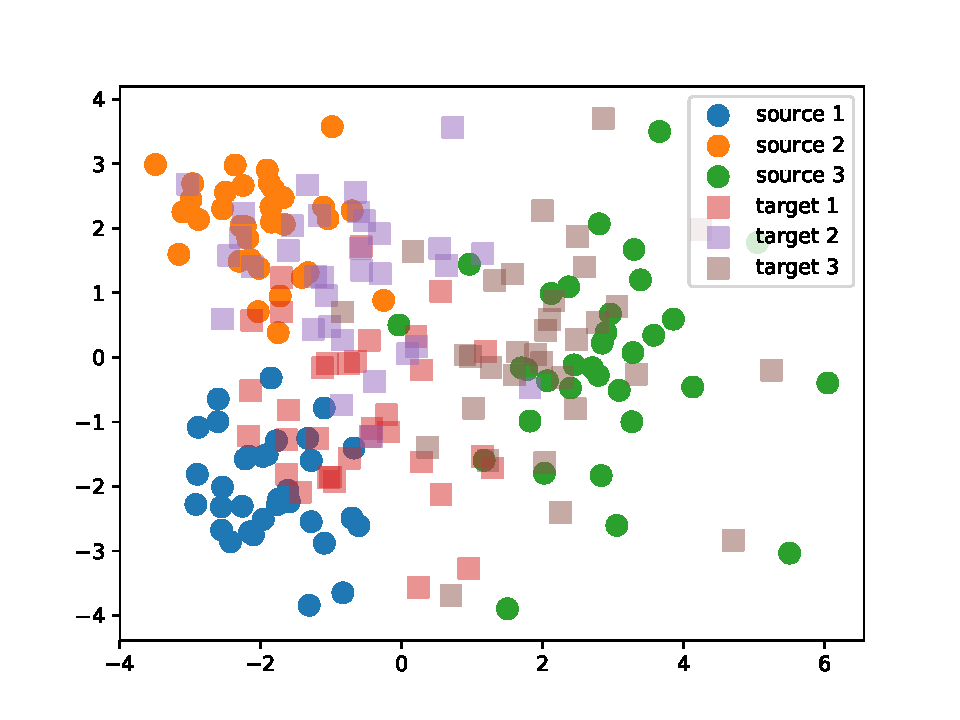
\includegraphics[width=6.cm]{./figs/da_toy_problem.pdf}~\hfill~\\
	~\hfill~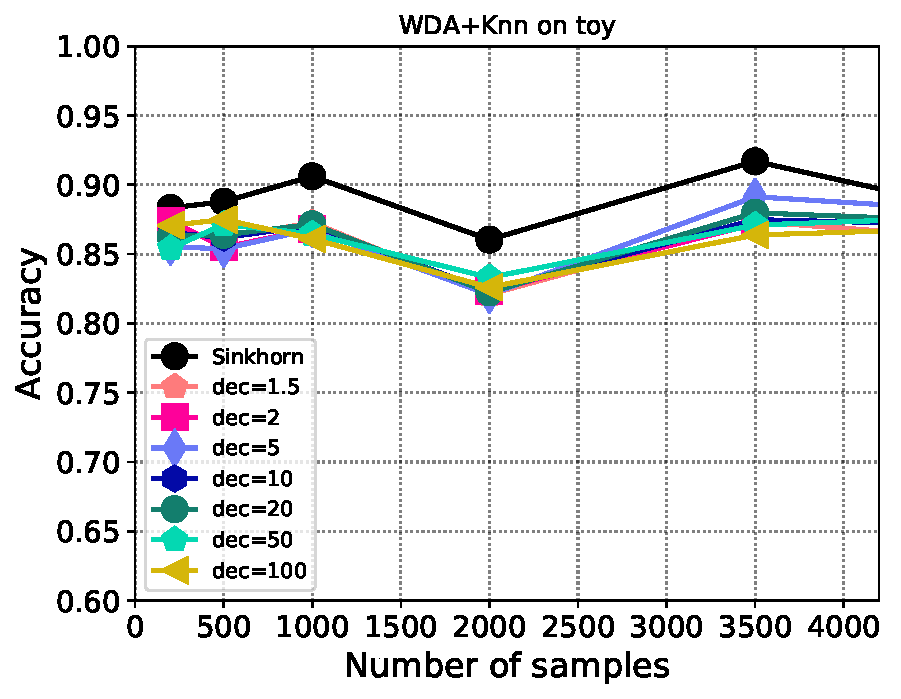
\includegraphics[width=6.cm]{./figs/wda_accur_toy.pdf}~\hfill~
	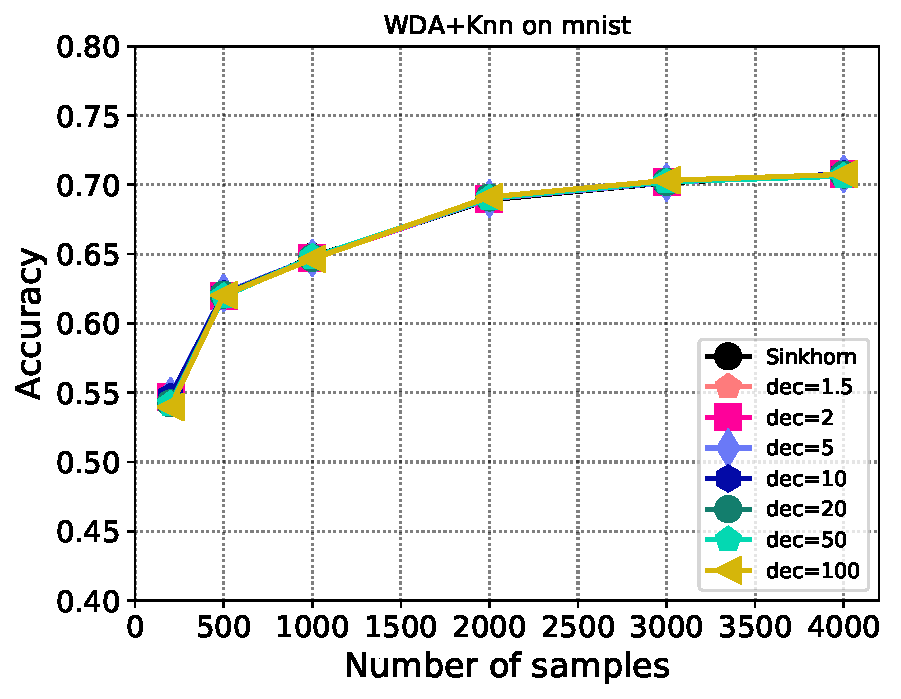
\includegraphics[width=6.cm]{./figs/wda_accur_mnist.pdf}~\hfill~\\
	\caption{Accuracy of a $1$-nearest-neighbour after WDA for the (left) toy problem.
		(right) MNIST). We note a slight loss of performance for the toy problem, whereas for MNIST, all approaches yield the same performance. 
		\label{fig:wda_gain}}
\end{figure*}

\begin{figure*}[htbp]
	\centering
	%~\hfill~	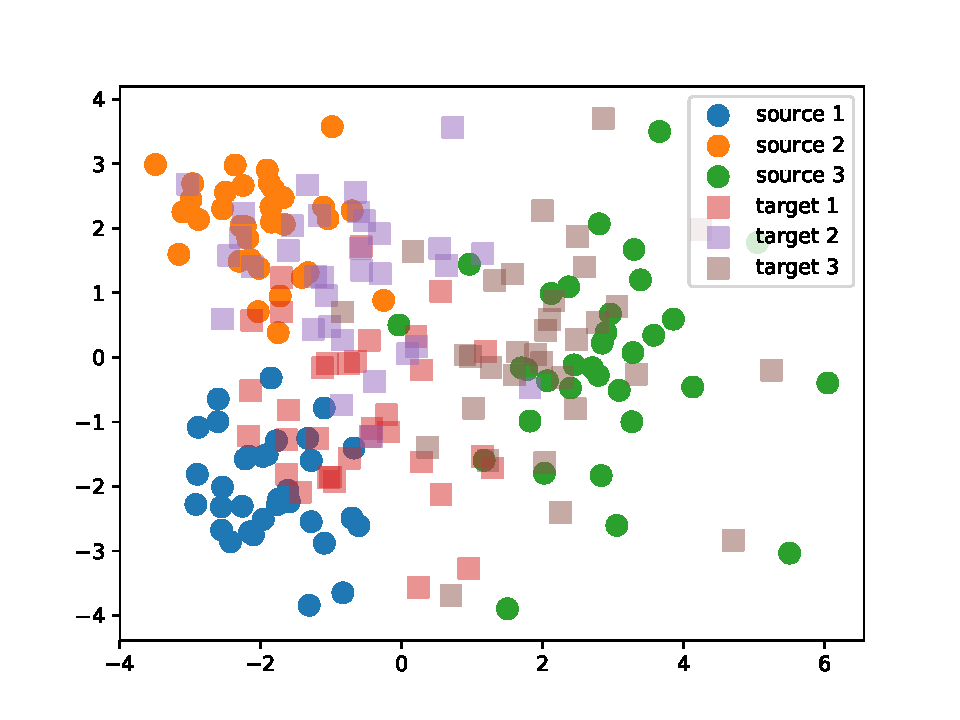
\includegraphics[width=6.cm]{./figs/da_toy_problem.pdf}~\hfill~\\
	~\hfill~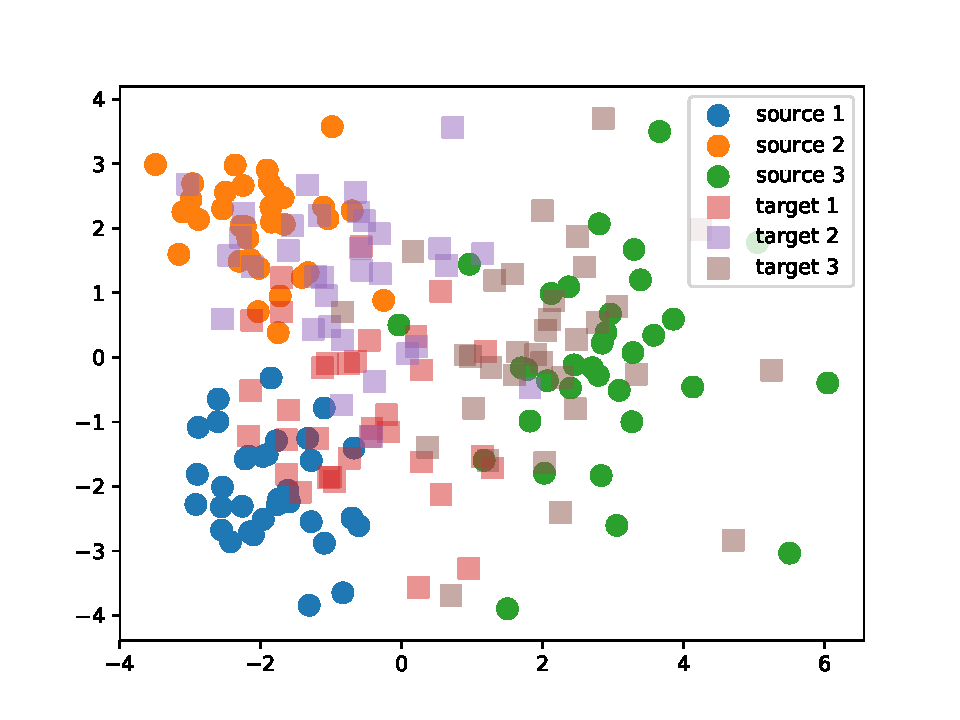
\includegraphics[width=6.cm]{./figs/da_toy_problem.pdf}~\hfill~
	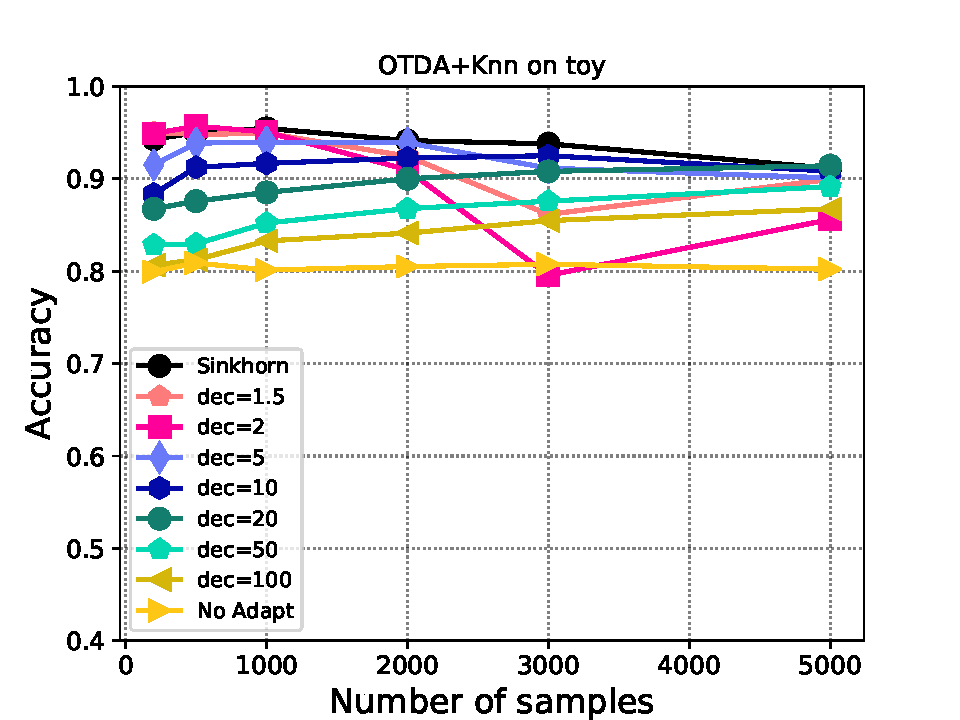
\includegraphics[width=6.cm]{./figs/da_accur_toy_regcl100.pdf}~\hfill~\\
	~\hfill~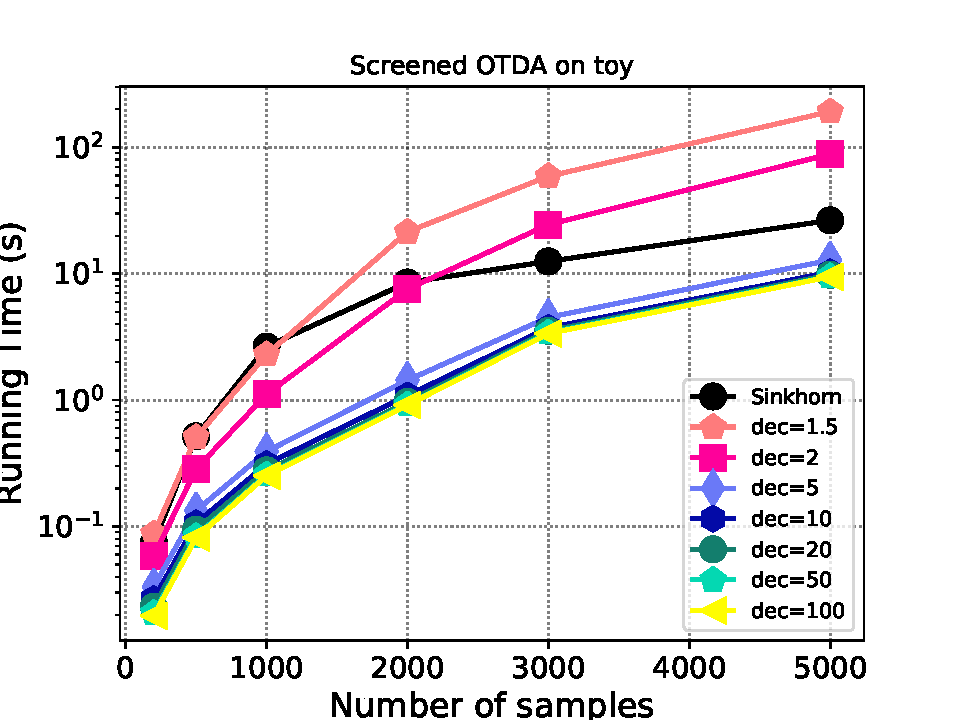
\includegraphics[width=6.cm]{./figs/da_time_toy_regcl100.pdf}
	~\hfill~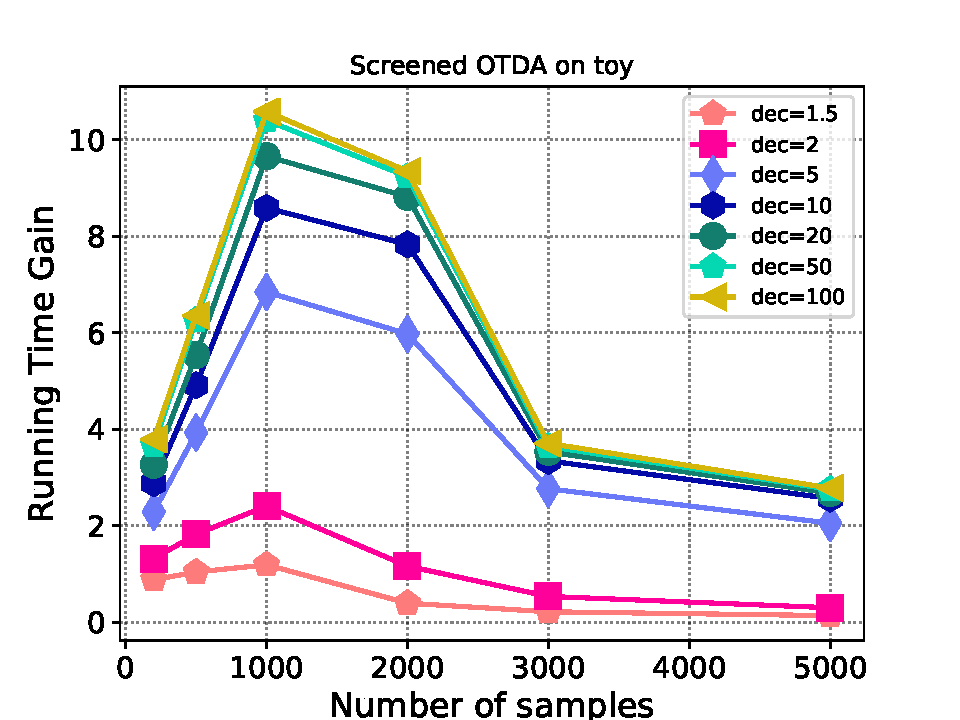
\includegraphics[width=6.cm]{./figs/da_gain_toy_regcl100.pdf}~\hfill~\\
	\caption{OT Domain Adaptation on a 3-class Gaussian toy problem. (top-left) Examples of source and target samples. (top-right) Evolution of the accuracy of a 1-nearest-neighbour classifier with respect to the number of samples. (bottom-left) Running time of the \emph{Sinkhorn} and \emph{Screenkhorn} for different decimation
	factors. (bottom-right). Gain in computation time. This toy problem is a problem in which classes are overlapping and distance between samples are rather limited. According to our analysis, this may be a situation in which \emph{Screenkhorn} may
	result in smaller computational gain. We can remark that with respect to the accuracy
	\emph{Screenkhorn} with decimation factors up to $10$ are competitive with \emph{Sinkhorn}, although a slight loss of performance. Regarding computational time, for this example, small decimation factors does not  result in gain. However for above  $5$-factor decimation, the gain goes from  $2$ to $10$ depending on
	the number of samples. 
	\label{fig:otda}}
\end{figure*}


\begin{figure*}[htbp]
	\centering
	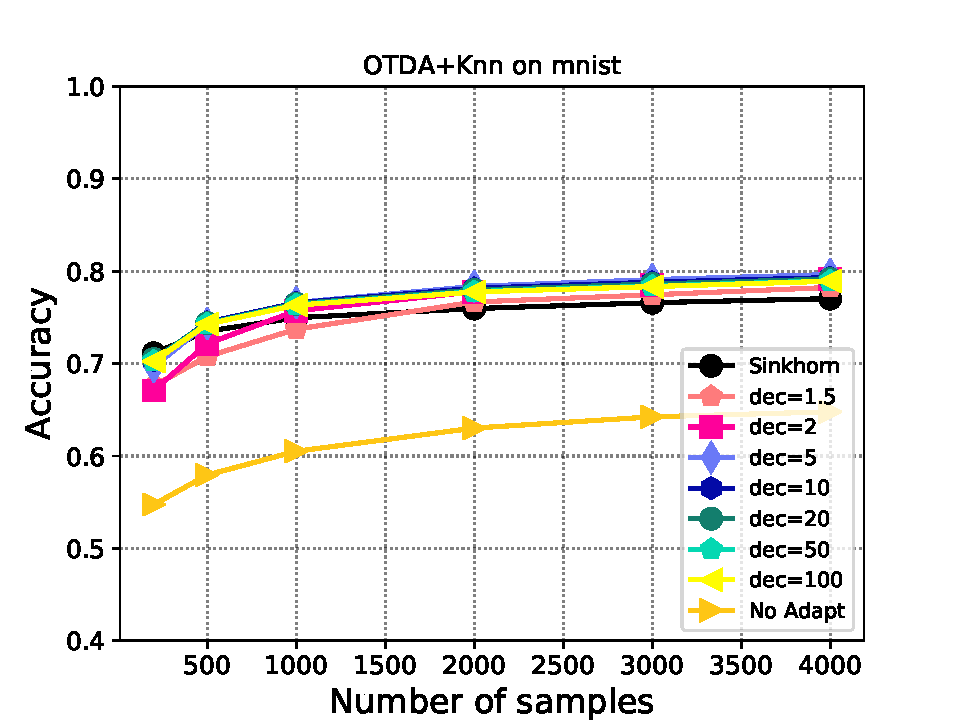
\includegraphics[width=6.5cm]{../../figure/da_accur_mnist_regcl1.pdf}
	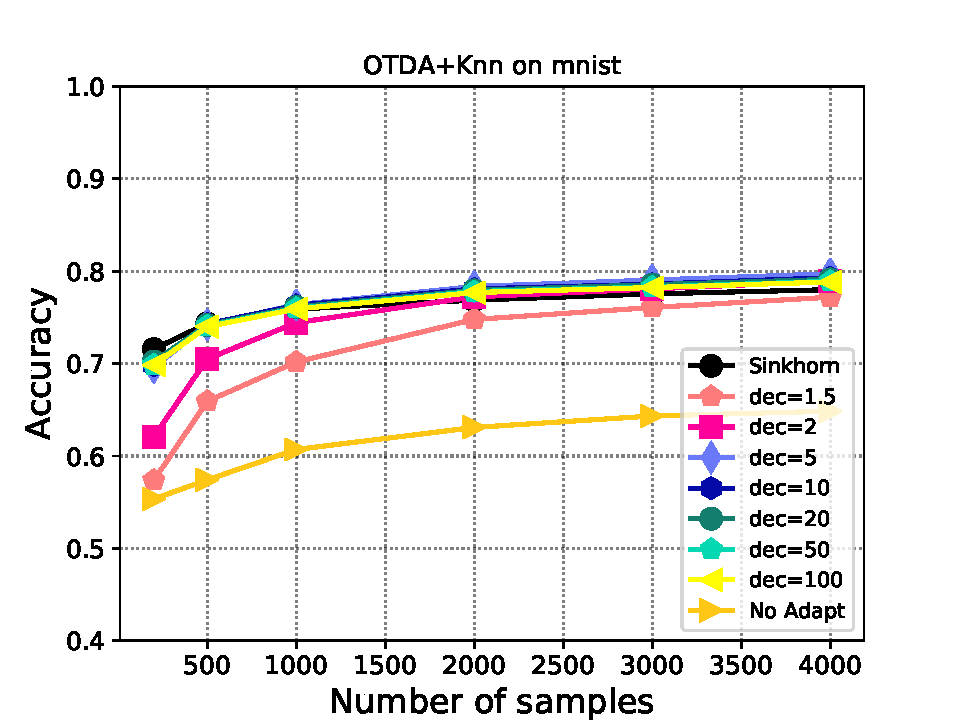
\includegraphics[width=6.5cm]{../../figure/da_accur_mnist_regcl10.pdf}
	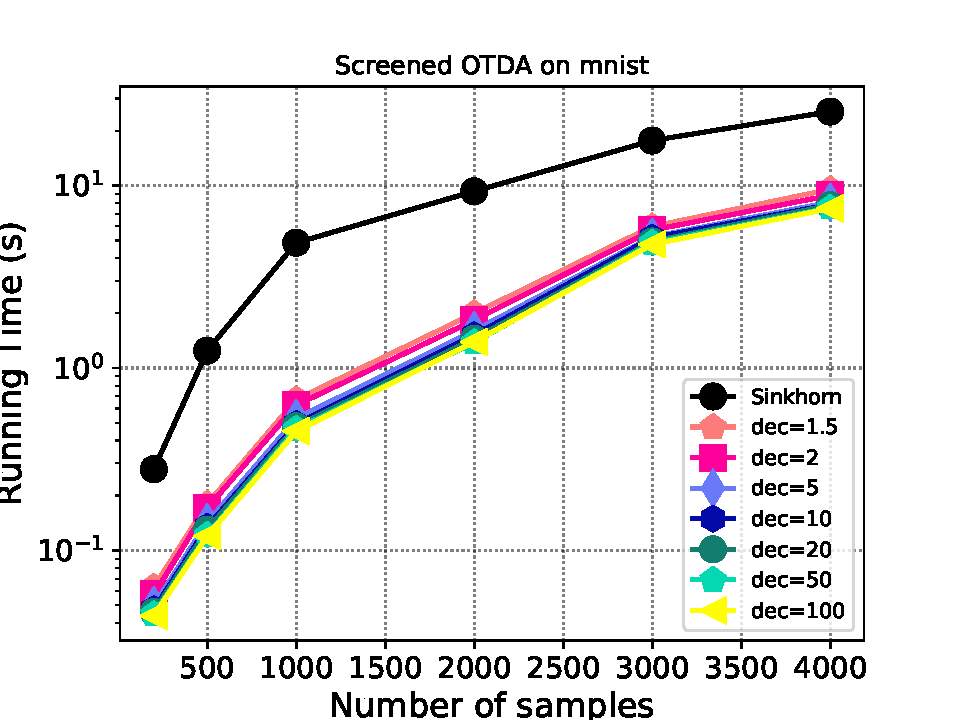
\includegraphics[width=6.5cm]{../../figure/da_time_mnist_regcl1.pdf}
	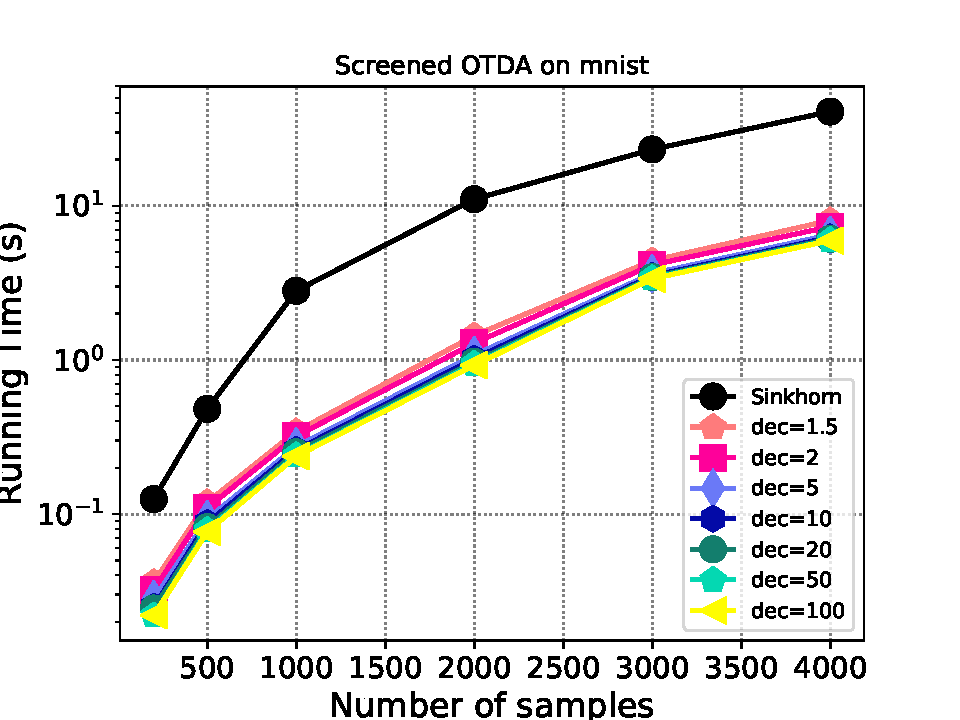
\includegraphics[width=6.5cm]{../../figure/da_time_mnist_regcl10.pdf}
	\caption{OT Domain adaptation MNIST to USPS : (top) Accuracy and (bottom) running time of Sinkhorn and \emph{Screenkhorn} for hyperparameter of the $\ell_{p,1}$ regularizer (left) $\lambda = 1$ and (right) $\lambda=10$. Note that this
	value impact of the ground cost of each Sinkhorn problem involved in the iterative algorithm. The accuracy panels
	also report the performance of a $1$-NN when no-adaptation is performed.  
	We remark that the strenght of the class-based has influence on the performance of \emph{Screenkhorn} given a decimation factor. For small value on the left, Screenkhorn slightly performs better than Sinkhorn, while for large value, some
	decimation factors leads to loss of performances.
	Regarding, running time, we can note that Sinkhorn is far less efficient than
	\emph{Screenkhorn}  with an order of magnitude for intermediate number of samples.
	\label{fig:otda:mnist:extra}}
\end{figure*}

